\documentclass[UTF8,a4paper,10.5pt]{ctexart}
\usepackage[a4paper,margin=1.75cm,headheight=14pt]{geometry}
\usepackage{amsmath,amssymb}
\usepackage{booktabs,longtable,tabularx,array}
\usepackage{xcolor}
\usepackage{hyperref}
\usepackage{fancyhdr}
\usepackage{microtype}
\usepackage{enumitem}
\usepackage{listings}
\usepackage{tikz}
\usetikzlibrary{arrows.meta,positioning,shapes.geometric,fit,backgrounds,calc}
\usepackage[
  pipeTables,
  fencedCode,
  texMathDollars,
  html,
  smartEllipses,
  hybrid
]{markdown}

\setCJKmainfont{Noto Serif CJK SC}
\setCJKsansfont{Noto Sans CJK SC}
\setCJKmonofont{Noto Sans Mono CJK SC}
\setmainfont{TeX Gyre Pagella}
\setsansfont{TeX Gyre Heros}
\setmonofont{Noto Sans Mono CJK SC}

\definecolor{DraNavy}{HTML}{17324D}
\definecolor{DraBlue}{HTML}{1F6AA5}
\definecolor{DraTeal}{HTML}{1D857D}
\definecolor{DraAmber}{HTML}{D38A19}
\definecolor{DraRed}{HTML}{B7493A}
\definecolor{DraLight}{HTML}{EFF5F8}
\definecolor{DraGray}{HTML}{5F6B76}
\definecolor{DraGreenLight}{HTML}{EAF5F1}
\definecolor{DraAmberLight}{HTML}{FFF5DF}

\hypersetup{
  colorlinks=true,
  linkcolor=DraBlue,
  urlcolor=DraBlue,
  citecolor=DraBlue,
  pdftitle={DRA Query 与环境扩容规划},
  pdfauthor={DRA Project · Codex × Kimi Design Review}
}

\pagestyle{fancy}
\fancyhf{}
\fancyhead[L]{\small\color{DraGray}DRA Query 与环境扩容规划}
\fancyhead[R]{\small\color{DraGray}Existing Sandbox → Multi-Domain vNext}
\fancyfoot[C]{\thepage}
\setlength{\parindent}{0pt}
\setlength{\parskip}{0.42em}
\setcounter{secnumdepth}{-1}
\setlist{nosep,leftmargin=2em}
\allowdisplaybreaks
\emergencystretch=3em
\sloppy

\lstdefinelanguage{text}{}
\lstset{
  basicstyle=\ttfamily\small,
  breaklines=true,
  breakatwhitespace=false,
  frame=single,
  rulecolor=\color{DraGray!35},
  backgroundcolor=\color{DraLight},
  columns=fullflexible,
  keepspaces=true,
  showstringspaces=false
}

\begin{document}

\begin{titlepage}
  \centering
  \vspace*{2.1cm}
  {\Huge\bfseries\color{DraNavy}DRA Query 与环境扩容规划\par}
  \vspace{0.55cm}
  {\LARGE\bfseries\color{DraBlue}基于现有沙盒的 vNext 路线图\par}
  \vspace{0.75cm}
  {\large Commerce · Community · Wikimedia\par}
  \vspace{0.15cm}
  {\large Science/Technical · Travel/Geo · Public Statistics\par}
  \vspace{1.15cm}

  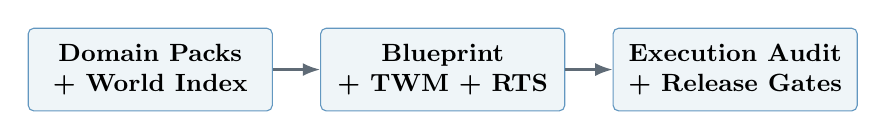
\begin{tikzpicture}[
    node distance=6mm,
    box/.style={rounded corners=2pt,draw=DraBlue!70,fill=DraLight,
      minimum width=3.1cm,minimum height=1.05cm,align=center,font=\small\bfseries},
    arrow/.style={-{Latex[length=2.2mm]},thick,color=DraGray}
  ]
    \node[box] (world) {Domain Packs\\+ World Index};
    \node[box,right=of world] (task) {Blueprint\\+ TWM + RTS};
    \node[box,right=of task] (run) {Execution Audit\\+ Release Gates};
    \draw[arrow] (world) -- (task);
    \draw[arrow] (task) -- (run);
  \end{tikzpicture}

  \vfill
  {\large Codex × Kimi 独立评审合并版\par}
  \vspace{0.25cm}
  {\large 2026-07-30 · Planning Draft v1.0\par}
  \vspace{0.7cm}
  {\small\color{DraGray}状态：规划文档；不构成正式 benchmark release 或 leaderboard claim\par}
\end{titlepage}

\tableofcontents
\clearpage

\section*{一页决策图}
\addcontentsline{toc}{section}{一页决策图}

\begin{tikzpicture}[
  x=1cm,y=1cm,
  phase/.style={rounded corners=2pt,draw=DraBlue!75,fill=DraLight,
    minimum width=2.65cm,minimum height=1.2cm,align=center,font=\scriptsize\bfseries},
  gate/.style={diamond,aspect=1.8,draw=DraAmber!90!black,fill=DraAmberLight,
    align=center,font=\scriptsize\bfseries,inner sep=1.5pt},
  arrow/.style={-{Latex[length=2mm]},thick,color=DraGray}
]
  \node[phase] (repair) at (1.5,4.4) {修复现有 Query\\资产隔离与治理};
  \node[phase] (e1) at (5.0,4.4) {E1/E3\\Commerce + Community};
  \node[phase] (e2) at (8.5,4.4) {E2\\W1M → Wfull};
  \node[phase] (e4) at (12.0,4.4) {E4\\Science + Travel + Stats};

  \node[gate] (worldgate) at (6.75,2.4) {World / Pack\\Gate};
  \node[phase,fill=DraGreenLight,draw=DraTeal] (mvp) at (3.0,0.4)
    {15 题方法学 MVP\\3 vertical × 5 shapes};
  \node[phase,fill=DraGreenLight,draw=DraTeal] (dev) at (6.75,0.4)
    {Dev-20\\Validity + Capacity};
  \node[phase,fill=DraGreenLight,draw=DraTeal] (formal) at (10.5,0.4)
    {Formal ≤ 60\\Reserve-16};

  \draw[arrow] (repair) -- (worldgate);
  \draw[arrow] (e1) -- (worldgate);
  \draw[arrow] (e2) -- (worldgate);
  \draw[arrow] (e4) -- (worldgate);
  \draw[arrow] (worldgate) -- (mvp);
  \draw[arrow] (mvp) -- (dev);
  \draw[arrow] (dev) -- node[above,font=\scriptsize]{双 ReleaseGate} (formal);
\end{tikzpicture}

\vspace{0.8em}
\begin{center}
\fcolorbox{DraRed!70}{DraAmberLight}{
  \parbox{0.91\textwidth}{
    \textbf{硬原则：}环境 scale-up 可以并行推进，但新 pack 未过 rights、coverage、
    agent-visible surface 与 delivery lineage 门之前，不得贡献正式题；
    ValidityGate 或 CapacityGate 失败时，应缩小 Formal 数量，不得降低标准。
  }
}
\end{center}

\clearpage
\markdownInput{dra-query-scaleup-input.md}

\end{document}
